\section{IMPLEMENTATION}
We implemented the simulation model using the programming language Python. Python was chosen over a simulation software as this problem does not have many components but each of these components has many backend behaviors that are not shown, hence simulation software such as Simul8 would not be as useful. Furthermore, Python is open-source hence it could be used and tested by anyone who needed it.

For this implementation, we did not use a simulation package, instead, we programmed each of the components such as queues, event handling and more. We decided to take this approach, instead of using a simulation library as SimPy, for three main reasons. Firstly, to manage all the priorities that each module has and use it accordingly. Secondly, this approach is easy to run several times the simulation without using multi-processing packages. Lastly, so we can have more control over the system and the debugging process.

This implementation is easily modified, as it is object-oriented. Hence, changing behavior of any of the components would be done by changing the methods of each object and obtaining in this manner the desired change. Furthermore, visualizing the simulation can be done through outputs in the terminal but, a graphical user interface was not implemented. 

On the contrary, it is easily used as all of the important aspects of the simulation are packed in different methods of the main class. In this manner, extracting information, testing the model and extracting the outputs are just done by calling those respective functions. 

\begin{figure}
    \centering
    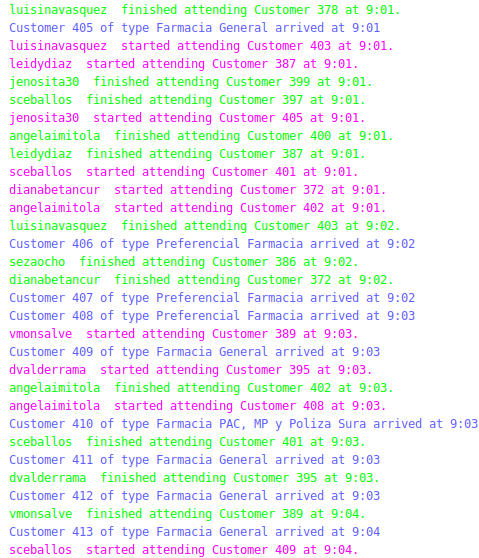
\includegraphics[scale=0.5]{files/screenshot_20191025_185940.png}
    \caption{Examples of output of the simulation.}
    \label{fig:implemen}
\end{figure}